\documentclass{article}

\usepackage[final]{style}
\usepackage[utf8]{inputenc} % allow utf-8 input
\usepackage[T1]{fontenc}    % use 8-bit T1 fonts
\usepackage{hyperref}       % hyperlinks
\usepackage{url}            % simple URL typesetting
\usepackage{booktabs}       % professional-quality tables
\usepackage{amsfonts}       % blackboard math symbols
\usepackage{nicefrac}       % compact symbols for 1/2, etc.
\usepackage{microtype}      % microtypography
\usepackage{verbatim}
\usepackage{graphicx}       % for figures

\title{Lecture \#9: Probability and Variational Inference Primer}

\author{
  Weixin Wang, Joo Gek Lim \\
  %Department of Computer Science\\
  %National University of Singapore\\
  %Singapore, S117417 %\\
  %\texttt{\{STUDENT1, STUDENT2, etc.\}@u.nus.edu} \\
}

\begin{document}

\maketitle

\section{Introduction}
In this lecture, we mainly study latent variable models, variational inference, amortized variational inference and generative models. The goal is to understand latent variable models and how to use variational inference.


\section{Probabilistic Latent Model}
\begin{figure}[h]
    \centering
	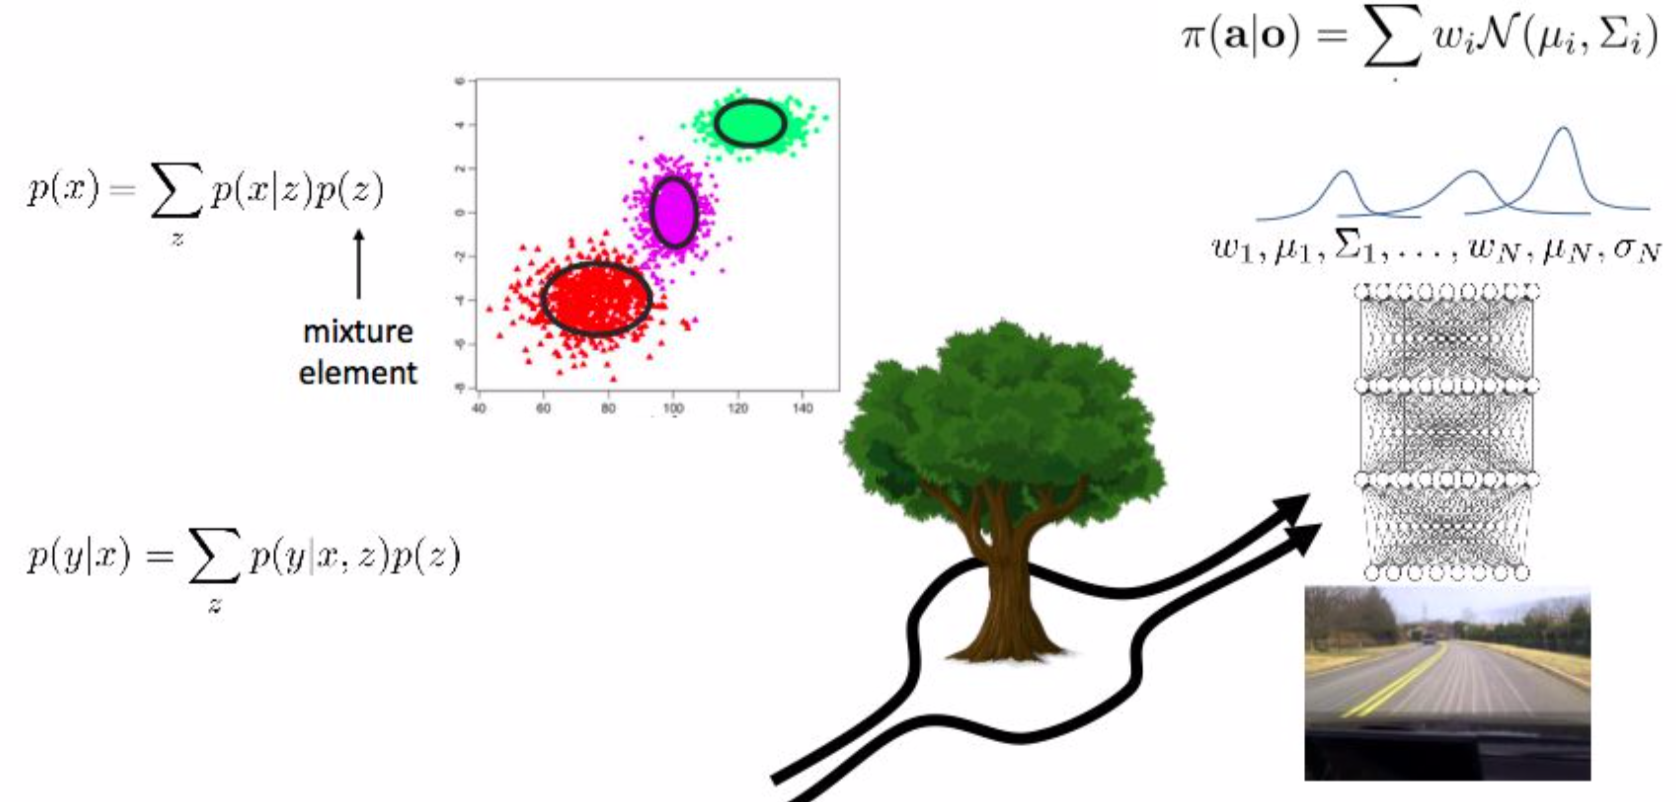
\includegraphics[width=0.8\textwidth]{fig/latent_model.png}
	\caption{The description of Latent variable models.}
	\label{fig:latent}
\end{figure}

Figure~\ref{fig:latent} shows an example of Gaussian mixture model where $z$ is the latent. 

\begin{figure}[h]
    \centering
	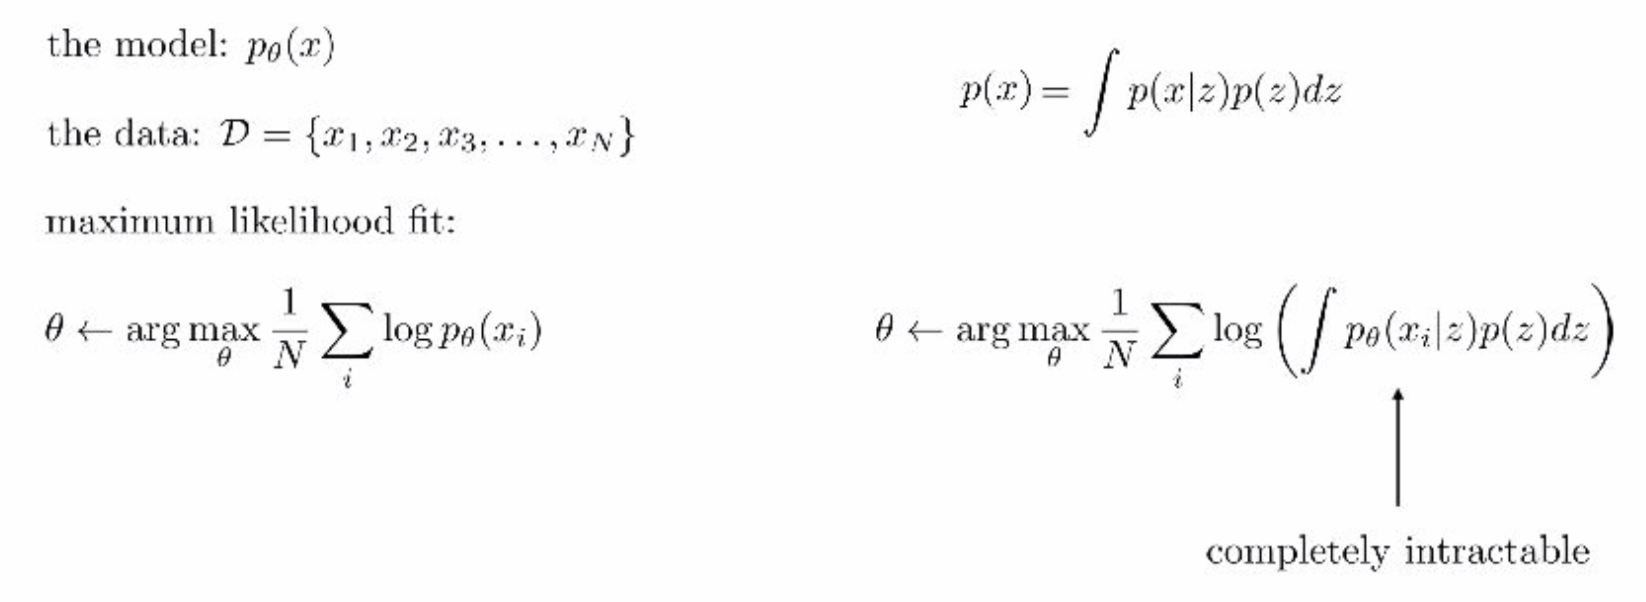
\includegraphics[width=0.8\textwidth]{fig/train_model.png}
	\caption{The description of Latent variable models.}
	\label{fig:train}
\end{figure}

\section{Variational Inference}
However, it is quite tough to train such latent variable models as described in Figure~\ref{fig:train}. Alternatively, we use approximate learning to learn the model. Here we first introduce KL-divergence, which is used to measure the difference between two distributions, as follows:

\begin{figure}[h]
    \centering
	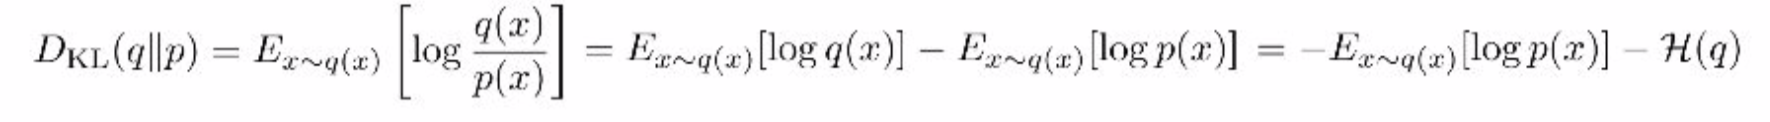
\includegraphics[width=\textwidth]{fig/kl.png}
\end{figure}

The variational inference is as follows:
\begin{figure}[h]
    \centering
	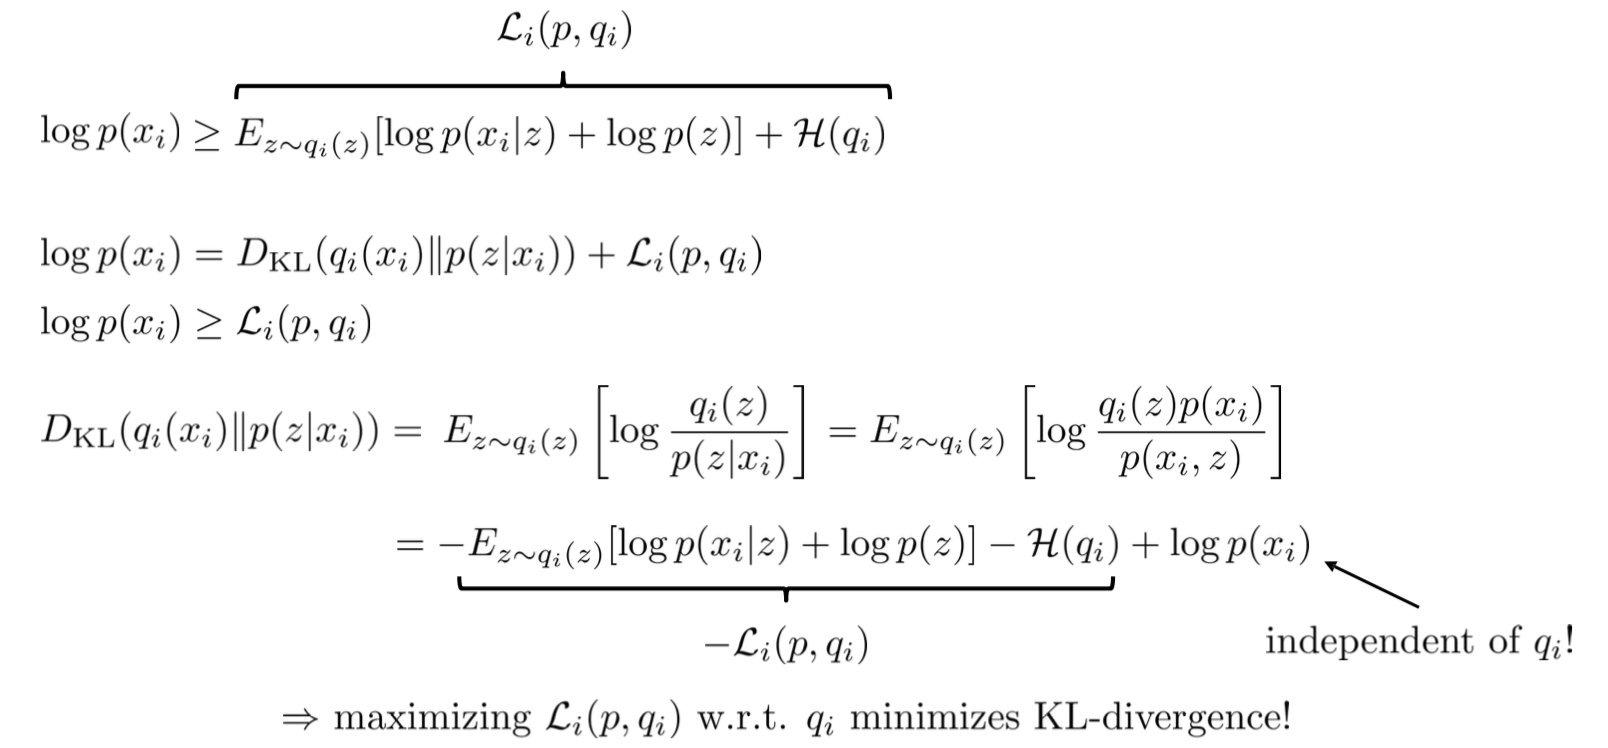
\includegraphics[width=\textwidth]{fig/variational_inference.png}
	\caption{The variational inference.}
\end{figure}
Our objective is to minimize KL-divergence.


\paragraph{Amortized Variational Inference}
\begin{figure}[h]
    \centering
	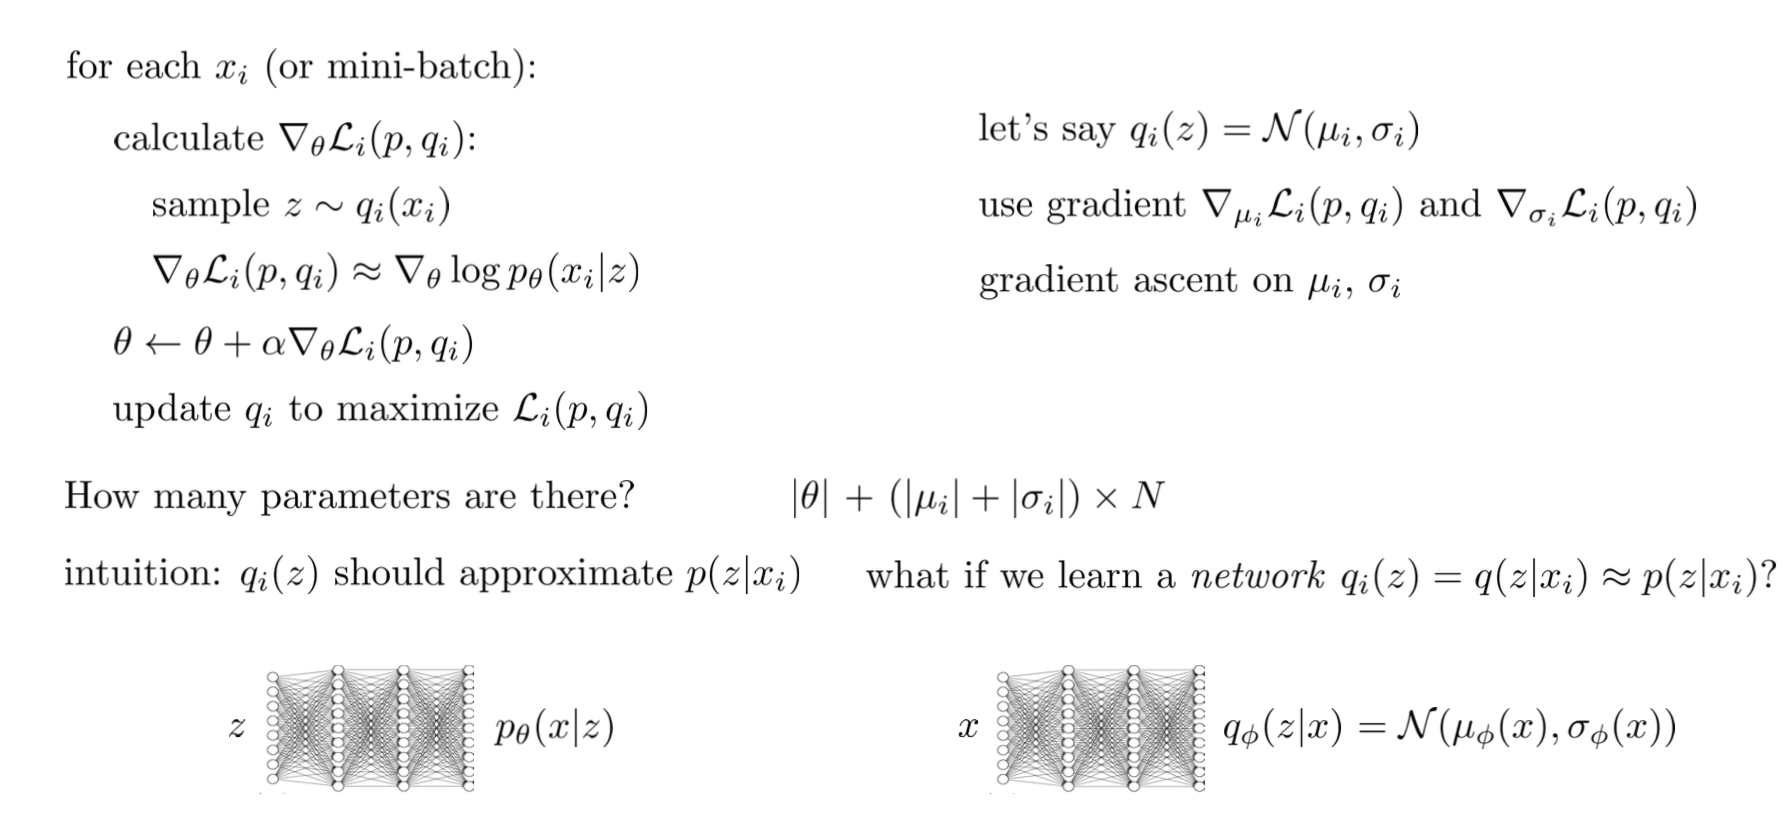
\includegraphics[width=\textwidth]{fig/vi_problem.png}
	\caption{The problem with variational inference.}
	\label{fig:problem}
\end{figure}
However, there will be a practical problem with varaiational inference as discussed in Figure~\ref{fig:problem}. Amortized variational inference is to, for example, a neural network that accepts the observation as input, and outputs the mean and variance parameter for the latent variable instead of optimizing a set of free parameters. We  then optimize the parameters of the neural network.
\begin{figure}[h]
    \centering
	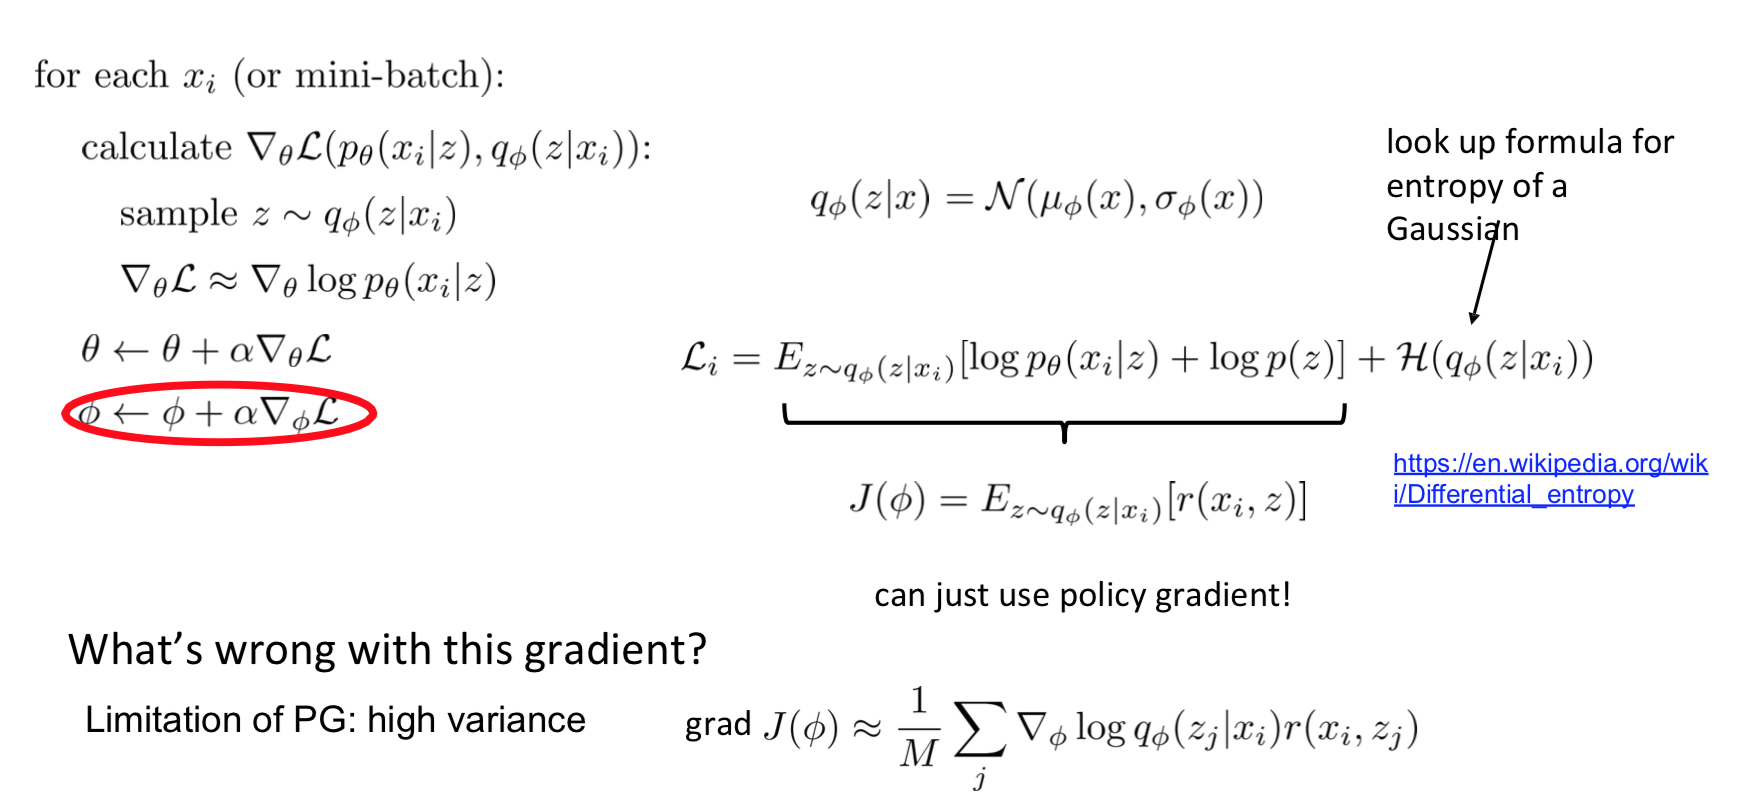
\includegraphics[width=\textwidth]{fig/amortized.png}
	\caption{Amartized varitional inference.}
	\label{fig:avi}
\end{figure}


\paragraph{Reparameterization Trick}

\begin{figure}[h]
    \centering
	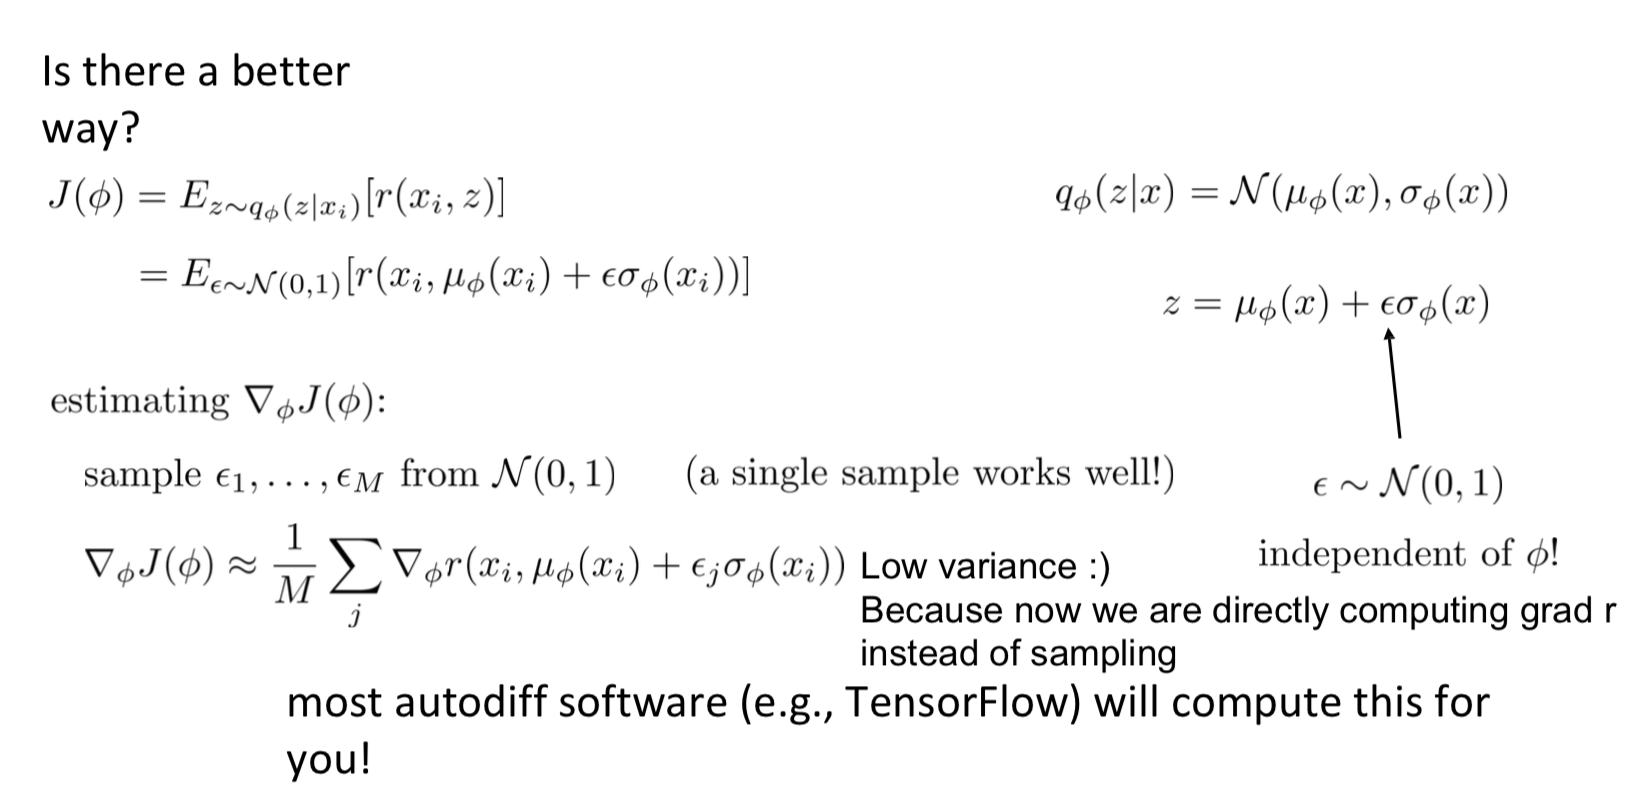
\includegraphics[width=\textwidth]{fig/trick.png}
	\caption{The reparameterization trick.}
\end{figure}
To solve the high variance problem as discussed in Figure~\ref{fig:avi}, we introduce the reparameterization trick. Compared with policy gradient, the reparameterization is very simple to implement and has low variance. However, it only works for continuous latent variables. While the policy gradient can handle both discrete and continuous variables. However, policy gradient has high variance and requires multiple samples and small learning rates.



\clearpage
\section{Variational Autoencoder}
\begin{figure}[h]
    \centering
	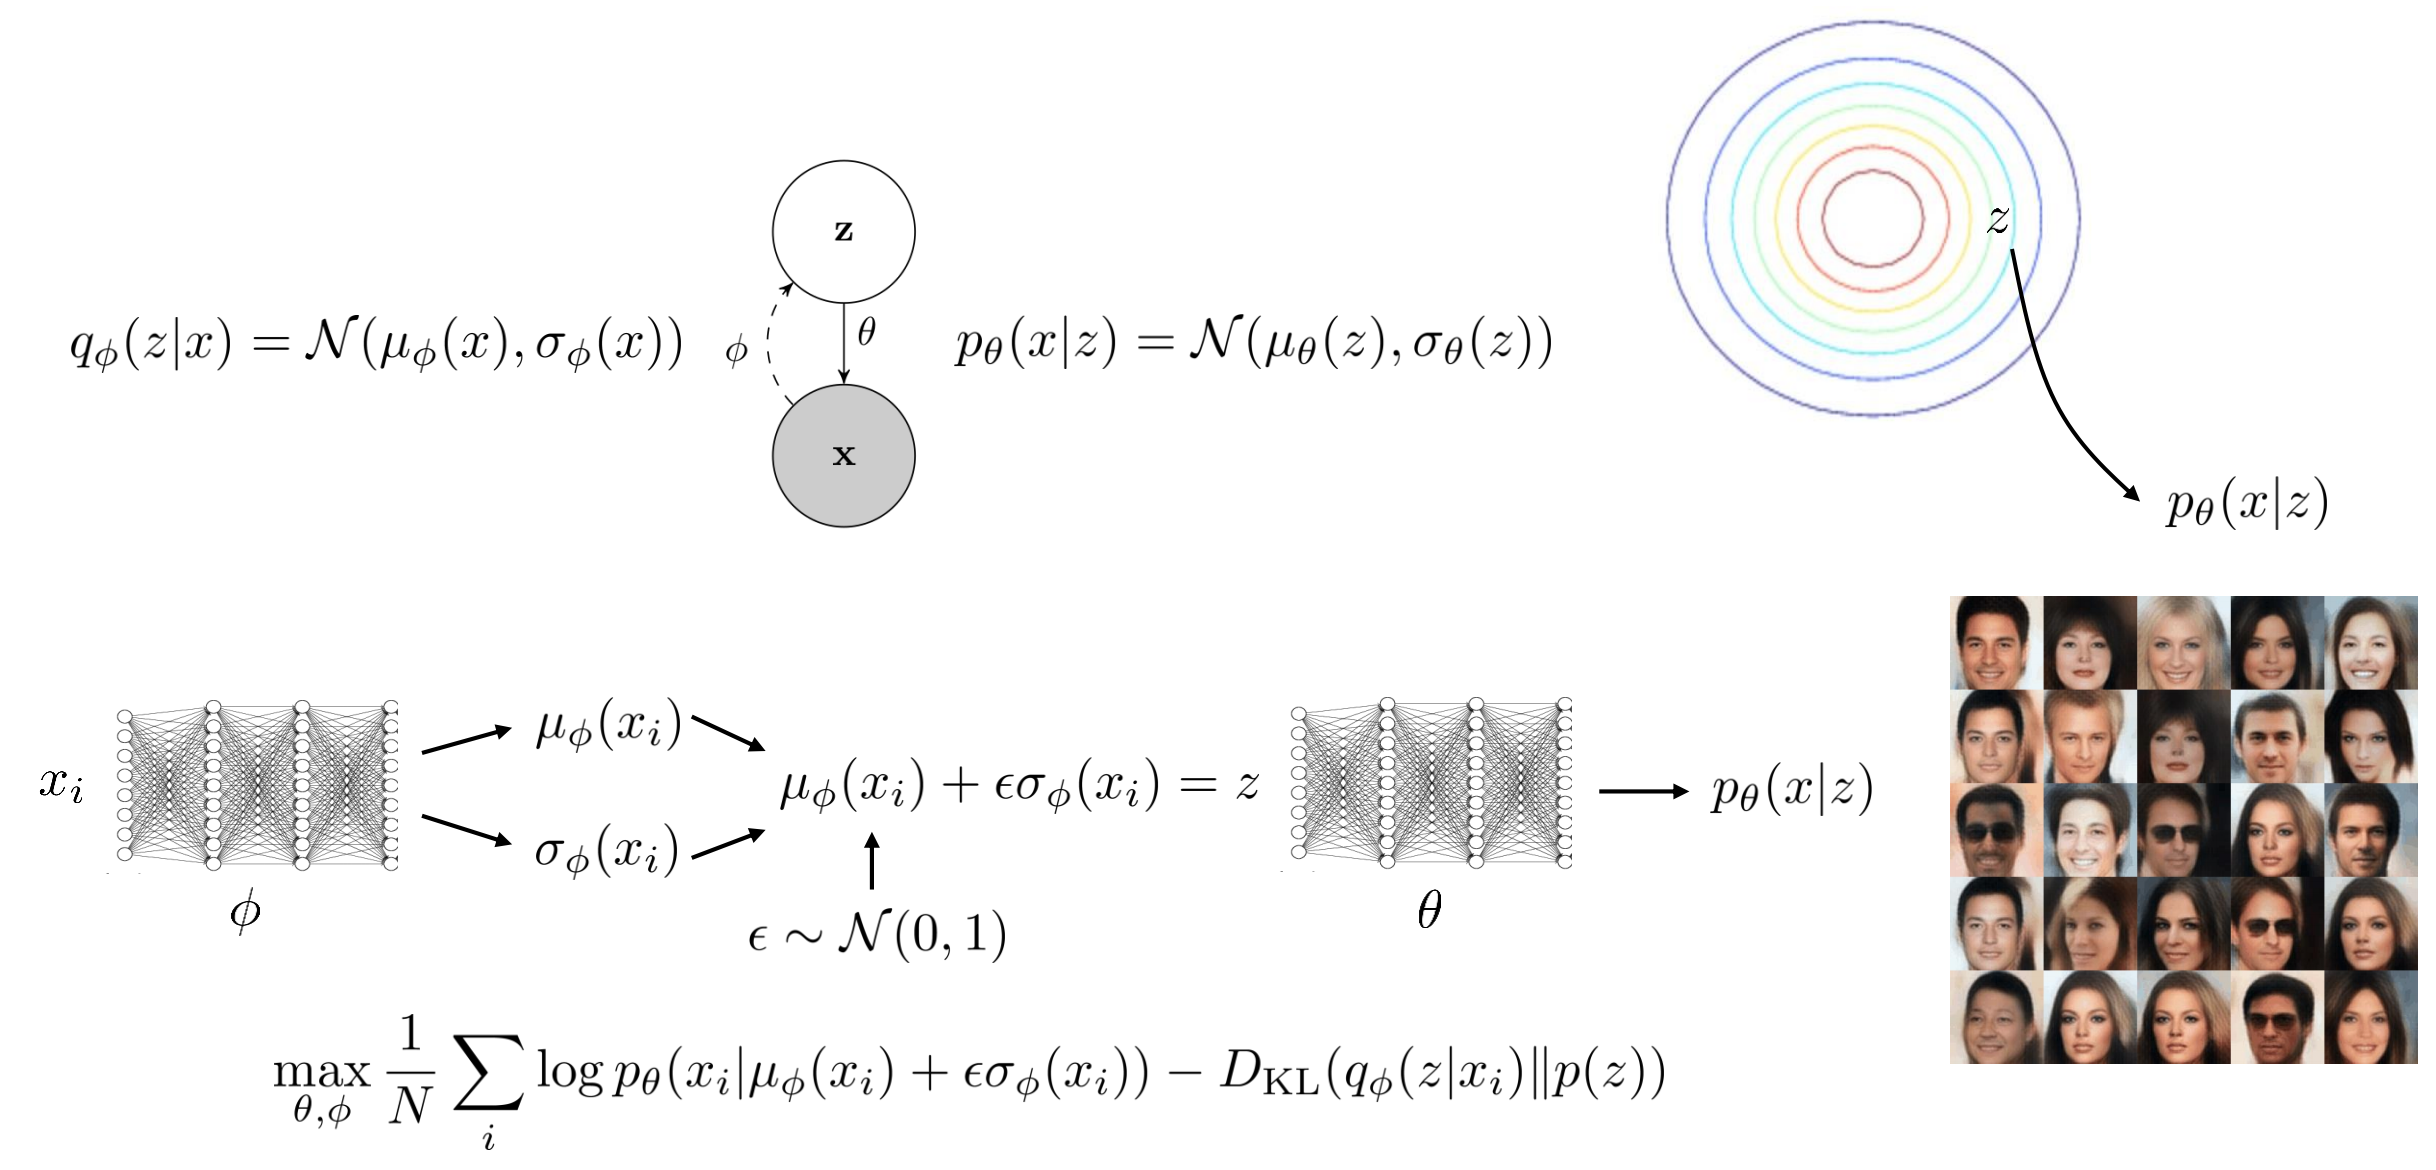
\includegraphics[width=\textwidth]{fig/vae.png}
	\caption{The illustration of Varitional Autoencoder.}
	\label{fig:vae}
\end{figure}


A variational autoencoder comprises an encoder, a decoder, and a loss function. As shown in Figure~\ref{fig:vae}, the encoder $q_{\phi}(z|x)$ takes as input $x$, and encodes $x$ into a latent representation $z$. While the decoder $p_{\theta}(x|z)$ takes as input the latent representation $z$ and predicts $x$.  The training objective consists of two parts where the first part is the expected log-likelihood and the second part is KL-divergence for measuring the information loss.
% References
\small
\bibliographystyle{plain}
\bibliography{bibliography}
\end{document}